\documentclass[10pt,compress]{beamer}
\usepackage{xspace}
\usepackage{tikz,pgfplots}
\usepackage{comment}

\definecolor{darkred}{HTML}{A60000}
\definecolor{lightblue}{HTML}{4B8EC8}
\definecolor{darkgreen}{HTML}{009000}
\definecolor{lightbrown}{HTML}{AB6402}
\definecolor{yellow9}{HTML}{EC811B}
\definecolor{blackish}{HTML}{23373B}

%% https://github.com/matze/mtheme.git
\usetheme{m}

\usepackage{amsmath,amsfonts,amssymb,amsthm}
\usepackage{xspace}
\usepackage{tikz}
\usepackage{graphicx}  % Required for including images

\usetikzlibrary{calc}
\usetikzlibrary{arrows,automata}
\usetikzlibrary{positioning}

\newcommand{\vs}{\vspace{5mm}}

\newcommand{\lattice}[3] {
  \coordinate (anchor) at (#1);
  \coordinate (b1) at (#2);
  \coordinate (b2) at (#3);
  \foreach \x in {0,1,2,3,4} {
    \foreach \y in {0,...,4} {
      \node [draw,circle,inner sep=1pt,fill] at ($(anchor) + {\x}*(b1) + {\y}*(b2)$) {};
    }
  }
}

\AtBeginSection[] {
  \begin{frame}
    \frametitle{Outline}
    \tableofcontents[sectionstyle=show/shaded,subsectionstyle=show/shaded]
  \end{frame}
}

\renewcommand{\vec}[1]{\mathbf{#1}\xspace}
\newcommand{\vol}[1]{\ensuremath{\textnormal{vol}\left(#1\right)}\xspace}

\newcommand{\A}{\vec{A}}
\newcommand{\s}{\vec{s}}
\newcommand{\ip}[2]{\langle #1, #2 \rangle}
\newcommand{\Zq}{\ensuremath{\Z_q}\xspace}
\newcommand{\vectorbound}{\ensuremath{\kappa}}
\newcommand{\secretbound}{\ensuremath{\nu}}
\newcommand{\E}{\ensuremath{\textnormal{E}}}
\newcommand{\Var}{\ensuremath{\textnormal{Var}}}
\newcommand{\Udist}[1]{\ensuremath{\mathcal{U}(#1)\xspace}}
\newcommand{\abs}[1]{\ensuremath{\|#1\|}\xspace}
\newcommand{\dotp}[2]{\ensuremath{\left\langle {#1},{#2}\right\rangle}\xspace}
\newcommand{\pq}{\ensuremath{\frac{p}{q}}}

\newcommand{\shortvec}[1]{\tilde{\mathbf{#1}}\xspace}
\renewcommand{\vec}[1]{\mathbf{#1}\xspace}
\newcommand{\cemph}[1]{{\color{yellow9}{\bf #1}}\xspace}
\newcommand{\chig}{\ensuremath{\chi_{\alpha,q}}}
\newcommand{\Z}{\ensuremath{\mathbb{Z}}\xspace}
\newcommand{\Zp}{\ensuremath{\mathbb{Z}_p}\xspace}
\newcommand{\Ldis}{L_{\mathbf{s},\chi}^{(n)}\xspace}
\newcommand{\sample}{\ensuremath{\leftarrow_{\$}}}
\renewcommand{\O}[1]{\ensuremath{{\mathcal{O}\left(#1\right)}}\xspace}
\newcommand{\round}[1]{\ensuremath{\left\lfloor{#1}\right\rceil}\xspace}
\newcommand{\Bdis}[1]{B_{\mathbf{s},\chi}(b,#1,p)\xspace}
\newcommand{\Bdissm}[1]{B_{small,\mathbf{s},\chi} (b,#1,p) \xspace}
\def\polyfactor{n\, \log_2^2 n}
\newcommand{\bigO}[1]{\ensuremath{\mathcal{O}\left(#1\right)}\xspace}
\def\DAG{D_{{\rm AG}}}

\title[On the concrete hardness of Learning with Errors]{On the concrete hardness of Learning with Errors}
\author[Martin R.\ Albrecht]{Martin R.\ Albrecht \texttt{@martinralbrecht}\\
 joint work with Rachel Player and Sam Scott}
\institute{Information Security Group Royal Holloway, University of London}
\date{ACE Seminar, UCL. May 7, 2015}
\begin{document}

\begin{frame}
  \maketitle
\end{frame}

\setcounter{tocdepth}{1}
\begin{frame}
  \frametitle{Outline}
  \tableofcontents
\end{frame}


\section{Learning With Errors}


\begin{frame}{Lattice-Based Cryptography}
  \begin{alertblock}{Lattice}
    A lattice is a discrete additive subgroup of $\mathbb{R}^m$.
  \end{alertblock} 
  \begin{alertblock}{Basis}
    Let $\vec{B} = \{ \vec{b}_1, ..., \vec{b}_m \}$ be a set of $m$ linearly independent vectors in $\mathbb{R}^m$. Then $L(\vec{B})=\{ \sum_{i=1}^{m} x_i \vec{b}_i \,|\, x_i \in \mathbb{Z}\}$ is the lattice generated by this basis.
  \end{alertblock} 
  \begin{alertblock}{Dual Lattice}
    Given a lattice $L(\vec{B}) \subset \mathbb{R}^m$, define its dual as $\{ \vec{x} \in \mathbb{R}^m \, | \, \vec{x} \vec{B} \in \mathbb{Z}^m  \}$. \\
  \end{alertblock}

  We’ll only use scaled-by-$q$ dual lattices, i.e.\  $\{ \vec{x} \in \Zq^m \, | \, \vec{x} \vec{B} \equiv \vec{0}  \}$
\end{frame}


\begin{frame}{Learning With Errors}
  The Learning with Errors (LWE) problem was defined by Oded Regev~\cite{STOC:Regev05}. 

  \begin{itemize}
  \item Suppose a public matrix $\vec{A}$ and a secret vector $\vec{s}$.
  \item If we were also given $\vec{b}=\vec{A}\vec{s}$ we could compute $\vec{s}$ by linear algebra.
  \item Now imagine this is noisy: $\vec{c}=\vec{A}\vec{s}+\vec{e}$ with $\vec{e}$ small.
  \item From $\vec{A}$ and  $\vec{c}$ can we find $\vec{s}$? Was $\vec{c}$ even computed this way?
  \end{itemize}
\end{frame}


\begin{frame}{Learning With Errors}
  Given $(\vec{A},\vec{c})$ with $\vec{c} \in \Zq^{m}$, $\vec{A} \in \Zq^{m \times n}$, $\vec{s} \in \Zq^{n}$ and $\vec{e} \in \Zq^{m \times \ell}$ do we have
  \[
    \left(\begin{array}{c}
            \\
            \\
            \\ 
            \vec{c} \\
            \\
            \\
            \\\end{array} 
        \right) = 
        \left(\begin{array}{ccc}
                \leftarrow & n & \rightarrow \\
                \\
                \\ 
                           & \vec{A} & \\
                \\
                \\
                \\
              \end{array} \right) 
            \times 
            \left(\begin{array}{c}
                    \\ 
                    \vec{s} \\
                    \\
                  \end{array}\right) 
                + \left(\begin{array}{c}
                          \\
                          \\
                          \\ 
                          \vec{e} \\
                          \\
                          \\
                          \\
                        \end{array}\right)
  \]
  or $\vec{c} \sample \Udist{\Zq^{m}}$.
\end{frame}


\begin{frame}
  \frametitle{Parameters}

  \begin{columns}
    \column{.5\textwidth}
    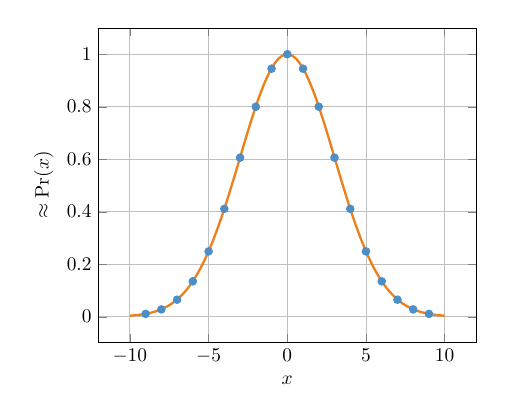
\begin{tikzpicture}[scale=0.7]
      \begin{axis}[
        domain=-10:10,
        grid=major,smooth,
        xlabel=$x$,
        ylabel=$\approx \textnormal{Pr}(x)$,
        ]
        \addplot[color=yellow9,very thick,samples=50,smooth]{exp(-(x^2)/18)};
        \addplot[only marks,color=lightblue] coordinates {
          (-9, 0.011)
          (-8, 0.028)
          (-7, 0.065)
          (-6, 0.135)
          (-5, 0.249)
          (-4, 0.411)
          (-3, 0.606)
          (-2, 0.800)
          (-1, 0.945)
          (0, 1.000)
          (1, 0.945)
          (2, 0.800)
          (3, 0.606)
          (4, 0.411)
          (5, 0.249)
          (6, 0.135)
          (7, 0.065)
          (8, 0.028)
          (9, 0.011)
        };
      \end{axis}
    \end{tikzpicture}
    \column{.50\textwidth}
    \begin{itemize}
    \item Parameters are: 
      \begin{itemize}
      \item dimension $n$, 
      \item modulus $q$ (e.g.\ $q \approx n^2$), 
      \item noise size $\alpha$ (e.g.\ $\alpha q \approx \sqrt{n}$),
      \item number of samples $m$.
      \end{itemize}

    \item Elements of $\vec{A}, \vec{s}, \vec{e}, \vec{c}$ are in $\mathbb{Z}_q$.
    \item $\vec{e}$ is sampled from a discrete Gaussian with width \[\sigma=\frac{\alpha q}{\sqrt{2 \pi}}.\]
    \end{itemize}
  \end{columns}
\end{frame}

\begin{frame}{Search and Decision}
  \begin{alertblock}{Search LWE}
    From samples $(\vec{A},\vec{c})$ recover $\vec{s}$.
  \end{alertblock}

  \vs{}

  \begin{alertblock}{Decision LWE}
    Determine if samples $(\vec{A},\vec{c})$ are LWE or uniformly random.
  \end{alertblock}

  \vs{}

  These problems are polynomial-time equivalent.

\end{frame}


\begin{frame}{LWE Normal Form}
  \begin{alertblock}{}
    Given samples \[(\vec{a},c)=(\vec{a},\langle\vec{a},\alert{\vec{s}}\rangle+ e) \in \Z_q^n \times \Z_q\] with $\vec{a} \gets \mathcal{U}(\Z_q^n)$, $e \gets D_{\alpha q,0}$ and $\vec{s} \in \Z_q^n$, we can construct samples \[(\vec{a}, c)=(\vec{a},\langle\vec{a},\alert{\vec{e}}\rangle+ e) \in \Z_q^n \times \Z_q\] 
    with $\vec{a} \gets \mathcal{U}(\Z_q^n)$, $e \gets D_{\alpha q, 0}$ and \alert{$\vec{e}$} such that all components \alert{$e_i \gets D_{\alpha q, 0}$} in polynomial time.
  \end{alertblock}
\end{frame}

\begin{frame}{Switching Moduli}
  \begin{alertblock}{}
    Let $(\vec{a},c) =(\vec{a}, \langle \vec{a}, \vec{s} \rangle + e) \in \Z_q^n \times \Z_q$ be an LWE sample and \[p \approx \sqrt{\frac{2\pi\, n}{12}} \cdot \frac{\sigma_s}{\alpha},\] where $\sigma_s$ is the standard deviation of components of the secret $\vec{s}$. If $p<q$ then $$\bigg(\round{\pq \cdot \vec{a}}, \round{\pq \cdot  c}\bigg) \textnormal{ in } \Z_p^n \times \Z_p$$ follows a distribution  close to an LWE distribution with parameters $n, \sqrt{2}\alpha, \alert{p}$.
  \end{alertblock}
\end{frame}


\begin{frame}{Why care?}
  Learning With Errors
  \begin{itemize}
  \item is assumed to be a hard problem like discrete logarithms, factoring, etc.
  \item reduces to hard problems on lattices, such as GapSVP.
  \item is assumed to have resistance against quantum computers, unlike discrete logarithms and factoring.
  \item is remarkably versatile for constructing cryptographic schemes.
  \end{itemize}

\end{frame}

\begin{frame}{Applications}
  \begin{alertblock}{Identity-based encryption~\cite{STOC:GenPeiVai08}}
    Ciphertexts are of the form
    $$ (\vec{p}, c) = (\A \vec{s} + \vec{e}, \vec{u} \cdot \s + e + b\cdot \lfloor q/2 \rfloor)  $$
    where $H(id) = \vec{u} = \vec{x}^T\A$ is the public key for the private key $\vec{x}$.

    Decryption is done by
    $$ c - \ip{\vec{x}}{\vec{p}} = -\ip{\vec{x}}{\vec{e}} + e + b \cdot \lfloor q/2 \rfloor. $$
  \end{alertblock}
\end{frame}


\begin{frame}{Applications}
  \begin{alertblock}{Fully homomorphic encryption~\cite{FOCS:BraVai11,AC:AFFP11}}
    Think of LWE encryptions \[(\vec{a}_i,c_i) =  (\vec{a}_i,\ip{\vec{a}_i}{\vec{s}} + e_i + b_i \cdot \lfloor q/2 \rfloor)\] as noisy linear polynomials \[-c_i + \sum a_{ij} x_j .\] Add, multiply and decrypt as usual.
  \end{alertblock}
\end{frame}


\begin{frame}{How hard is LWE?}
  
  Given $n$ (and $\alpha$, $q$) how many operations does it take to solve? 

  \begin{itemize}
  \item \alert{Problem 1.} Algorithms/attacks are not well understood in terms of concrete running times.
    \begin{itemize}
    \item Runtimes are given asymptotically.
    \item Algorithms are better in practice than the theoretical bounds.
    \item Many heuristic assumptions.
    \end{itemize} 

  \item \alert{Problem 2.} Many variables
    \begin{itemize}
    \item dimension, modulus, secret size
    \item distribution of the secret
    \item number of samples available to an attacker
    \item variants of the problem (e.g.\ small secrets, BinaryError-LWE)
    \end{itemize}
  \end{itemize}
\end{frame}

\begin{frame}{What do people do currently?}
  Often, in the literature, the following assumptions were made when estimating concrete security of an LWE-based scheme:

  \begin{itemize}
  \item the best attack is a lattice-based \alert{distinguishing attack};
  \item \alert{BKZ} runs in roughly the time given in~\cite{RSA:LinPei11};
  \item the use of a \alert{small secret} makes no difference for attacks.
  \end{itemize} 

  All three of these assumptions turn out not to be correct.

\end{frame}


\begin{frame}{So, what did we do?}
  \begin{itemize}
  \item Overview the \alert{strategies} for attacking LWE.{}
  \item Analyse and present \alert{running times}. 
  \item Produce \alert{concrete estimates} for attack timings for parameters sets.
  \end{itemize} 

  The estimation code is available as a Sage module.
  \end{frame}

\section{Strategies and Algorithms}

\begin{frame}{Strategies for Solving LWE}
  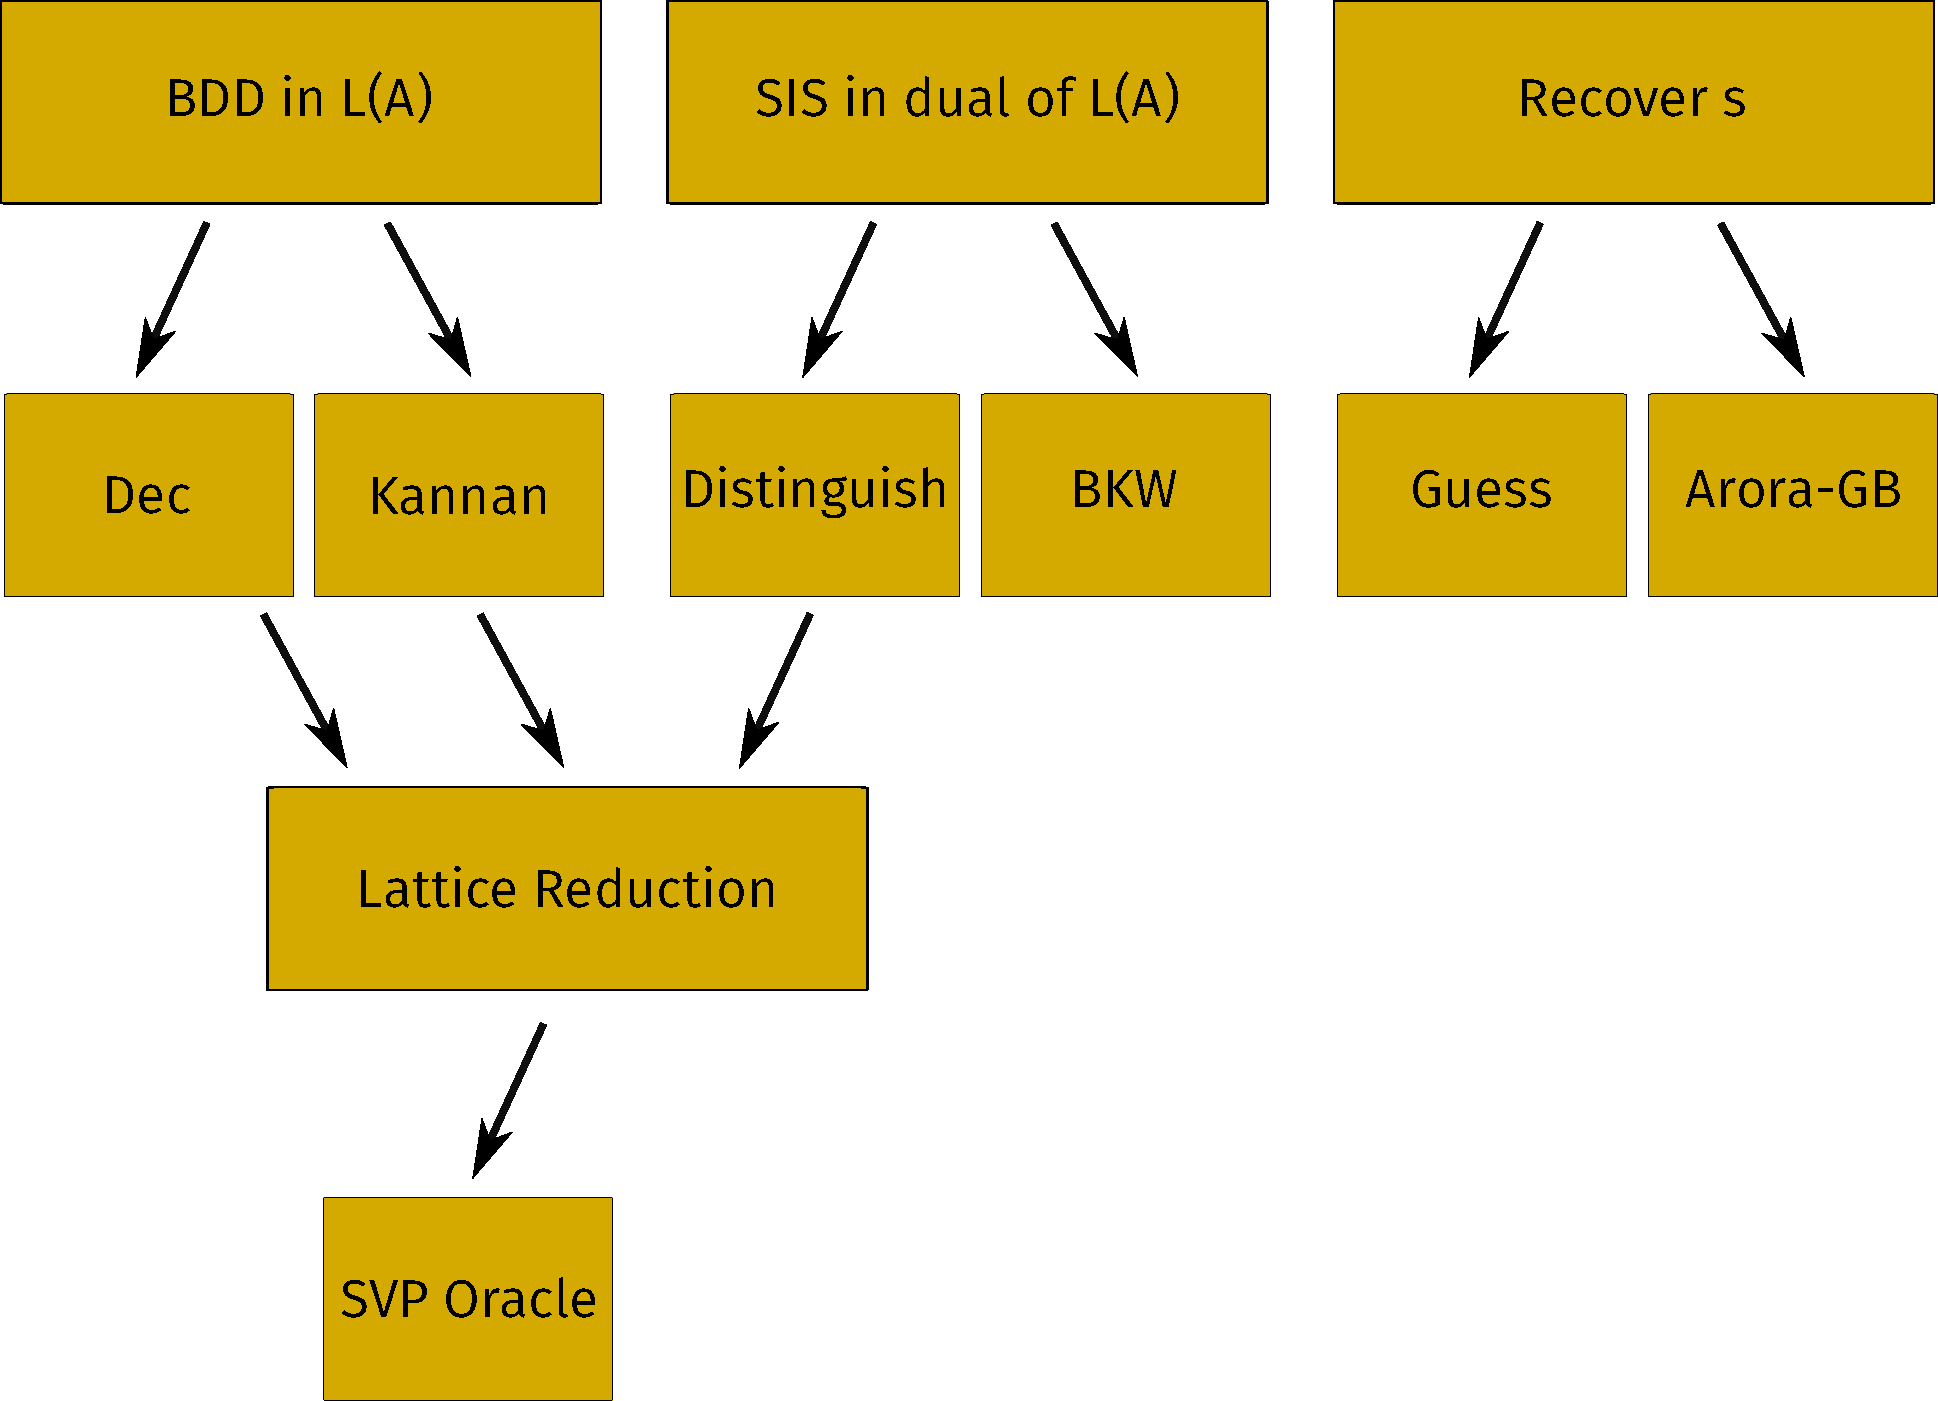
\includegraphics[width=0.9\textwidth]{overviewflowchart.pdf}
\end{frame}


\begin{frame}{Arora-GB}
  \framesubtitle{Strategy 1: Recover $\vec{s}$}

  \begin{columns}
    \column{0.6\textwidth}
    \begin{tikzpicture}[scale=0.9]
      \begin{axis}[%every axis plot post/.append style=,
        domain=-13:13,
        ] % extend the axes a bit to the right and top
        \addplot[color=mLightBrown,very thick,samples=50,smooth]{exp(-(x^2)/18)};
        \addplot[very thick,color=mDarkBrown] coordinates { (-12,0) (-12,1.0) };
        \addplot[very thick,color=mDarkBrown] coordinates { (12,0) (12,1.0) };  
      \end{axis}
    \end{tikzpicture}
    \column{0.4\textwidth}  
    \begin{itemize}
    \item The error is from a small subset of $\Zq$, say, $(-\tau \cdot \sigma,\dots,\tau \cdot \sigma)$
    \item Each candidate gives rise to one linear equation.
    \item Construct equations of degree $2\,\tau \cdot \sigma +1$ encoding that one of these linear equations must hold.
    \item Solve the system using Gröbner bases.
    \end{itemize}
  \end{columns}
\end{frame}


\begin{frame}{Arora-GB}
  \framesubtitle{Strategy 1: Recover $\vec{s}$}
  \alert{Arora-Ge} (Linearisation) with $\sigma = \sqrt{n}$
  \begin{center}
    \Large $\bigO{2^{\omega\,n\log( 8n \log n) - \omega n \log n}}$
  \end{center}
  \phantom{under some regularity assumption.}

  \alert{Gröbner Bases} with $\sigma = \sqrt{n}$
  \begin{center}
    \Large $\bigO{2^{2.82\,\omega\,n}}$
  \end{center}
  under some regularity assumption.

  \vs{}

  \begin{thebibliography}{foobar}
  \bibitem[ACFP14]{EPRINT:ACFP14}
    M.A., Carlos Cid, Jean-Charles Faug{\`e}re, and Ludovic Perret.
    \newblock Algebraic algorithms for {LWE}.
    \newblock Cryptology ePrint Archive, Report 2014/1018, 2014.
    \newblock \url{http://eprint.iacr.org/2014/1018}.
  \end{thebibliography}

\end{frame}


\begin{frame}{What is SIS?}
  \framesubtitle{Strategy 2: SIS}
  \begin{alertblock}{Short Integer Solutions (SIS)}
    Given $q \in \mathbb{Z}$, a matrix $\vec{B}$, and $t < q$; find $\vec{y}$ with $0 < \| \vec{y} \| \leq t$ and
    \[\vec{y} \vec{B} \equiv  \vec{0} \pmod{q}.\]
  \end{alertblock}

  
  \begin{itemize}
  \item Recall the dual lattice: $L^* = \{ \vec{x} \in \mathbb{R}^m \enspace | \enspace \vec{x} \vec{B} \in \mathbb{Z}^m \}$. 
  \item Then the scaled dual lattice, $qL^*$ has the property that $ \vec{x} \vec{B} \equiv 0 \pmod{q}$ for all $\vec{x} \in qL^*$. 
  \item Therefore, a short vector of $qL^*$ is equivalent to solving SIS on $\vec{B}$.
  \end{itemize}

\end{frame}

\begin{frame}{Strategy}
  \framesubtitle{Strategy 2: SIS}
  \begin{itemize}
  \item Find a short $\vec{y}$ solving SIS on $\vec{A}$. 
  \item Given LWE samples $\vec{A}, \vec{c}$ where either $\vec{c} = \A\s + \vec{e}$ or $\vec{c}$ uniformly random. 
  \item Compute $\ip{\vec{y}}{\vec{c}}$. 
    \begin{itemize}
    \item If $\vec{c} = \A\s + \vec{e}$, then $\ip{\vec{y}}{\vec{c}} = \ip{\vec{y}\A}{\s} + \ip{\vec{y}}{\vec{e}} \equiv \ip{\vec{y}}{\vec{e}} \pmod{q}$.
    \item If $\vec{c}$ is uniformly random, so is $\ip{\vec{y}}{\vec{c}}$.
    \end{itemize} 
  \item If $\vec{y}$ is sufficiently short, since $\vec{e}$ is also small, then $\ip{\vec{y}}{\vec{e}}$ will also be short, and can be distinguished from uniform values.

  \end{itemize}
\end{frame}


\begin{frame}{Distinguish (Lattice Reduction)}
  \framesubtitle{Strategy 2: SIS}

  A \alert{reduced lattice} basis is made of short vectors, in particular the first vector.
  \begin{enumerate}
  \item Construct a basis of the dual from the instance.
  \item Feed to a lattice reduction algorithm to obtain short vectors $\vec{v}_i$.
  \item Check if $\vec{v}_i\, \vec{A}$ are small.
  \end{enumerate}

  \begin{thebibliography}{99}
  \bibitem[MR09]{PQCBook:MicReg09}
    Daniele Micciancio and Oded Regev.
    \newblock Lattice-based cryptography.
    \newblock In Bernstein et~al. \cite{PQCBook}, pages 147--191.
  \end{thebibliography}
\end{frame}


\begin{frame}[fragile]{BKW Algorithm}
  \framesubtitle{Strategy 2: SIS}

  We revisit Gaussian elimination:
  \begin{eqnarray*}
    & & \left(
        \begin{array}{c|c|ccc|c}
          \bold{a}_{11} & \bold{a}_{12} & \bold{a}_{13} & \cdots & \bold{a}_{1n} & c_1\\
          \bold{a}_{21} & \bold{a}_{22} & \bold{a}_{23} & \cdots & \bold{a}_{2n} & c_2\\
          \vdots & \vdots & \vdots & \ddots & \vdots & \vdots\\
          \bold{a}_{m1} & \bold{a}_{m2} & \bold{a}_{m3} & \cdots & \bold{a}_{mn} & c_{m}
        \end{array}
                                                                                   \right)
  \end{eqnarray*}

  \begin{eqnarray*}
    & \overset{?}{=} & \left(
                       \begin{array}{c|c|ccc|c}
                         \bold{a}_{11} & \bold{a}_{12} & \bold{a}_{13} & \cdots & \bold{a}_{1n} & \dotp{\vec{a}_1}{\vec{s}} + \vec{e}_1\\
                         \bold{a}_{21} & \bold{a}_{22} & \bold{a}_{23} & \cdots & \bold{a}_{2n} & \dotp{\vec{a}_2}{\vec{s}} + \vec{e}_2\\
                         \vdots & \vdots & \vdots & \ddots & \vdots & \vdots\\
                         \bold{a}_{m1} & \bold{a}_{m2} & \bold{a}_{m3} & \cdots & \bold{a}_{mn} & \dotp{\vec{a}_m}{\vec{s}} + \vec{e}_m
                       \end{array}\right)
  \end{eqnarray*}
\end{frame}

\begin{frame}[fragile]{BKW Algorithm}
  \framesubtitle{Strategy 2: SIS}
  \begin{eqnarray*}
    & \Rightarrow  & \left(
                     \begin{array}{c|c|ccc|l}
                       \bold{a}_{11} & \bold{a}_{12} & \bold{a}_{13} & \cdots & \bold{a}_{1n} & \dotp{\vec{a}_1}{\vec{s}} + \vec{e}_1\\
                       0 & \tilde{\bold{a}}_{22} & \tilde{\bold{a}}_{23} & \cdots & \tilde{\bold{a}}_{2n} & \dotp{\shortvec{a}_2}{\vec{s}} + \vec{e}_2 - \alert{\frac{\bold{a}_{21}}{\bold{a}_{11}}\vec{e}_1}\\
                       \vdots & \vdots & \ddots & \vdots & \vdots\\
                       0 & \tilde{\bold{a}}_{m2} & \tilde{\bold{a}}_{m3} & \cdots & \tilde{\bold{a}}_{mn} & \dotp{\shortvec{a}_m}{\vec{s}} + \vec{e}_m - \alert{\frac{\bold{a}_{m1}}{\bold{a}_{11}}\vec{e}_1}
                     \end{array}\right)\phantom{\Longrightarrow}
  \end{eqnarray*}

  \begin{itemize}
  \item $\frac{\bold{a}_{i1}}{\bold{a}_{11}}$ is essentially random in $\Z_q$ wiping all ``smallness''.
  \item If $\frac{\bold{a}_{i1}}{\bold{a}_{11}}$ is 1 noise-size doubles because of the addition.  
  \end{itemize}
\end{frame}

\begin{frame}[fragile]{BKW Algorithm}
  \framesubtitle{Strategy 2: SIS}
  We considering $a \approx \log n$ `blocks' of $b$ elements each.

  \begin{equation*}
    \left(
      \begin{array}{cc|ccc|c}
        \bold{a}_{11} & \bold{a}_{12} & \bold{a}_{13} & \cdots & \bold{a}_{1n} & c_0\\
        \bold{a}_{21} & \bold{a}_{22} & \bold{a}_{23} & \cdots & \bold{a}_{2n} & c_1\\
        \vdots & \vdots & \vdots & \ddots & \vdots & \vdots\\
        \bold{a}_{m1} & \bold{a}_{m2} & \bold{a}_{m3} & \cdots & \bold{a}_{mn} & c_{m}
      \end{array}
    \right)
  \end{equation*}
\end{frame}

\begin{frame}[fragile]{BKW Algorithm}
  \framesubtitle{Strategy 2: SIS}
  For each block we build a table of all $q^b$ possible values indexed by $\Z_q^b$.

  \begin{equation*}
    T^0 = \left[ 
      \begin{array}{ll|ccc|c}
        -\lfloor\frac{q}{2}\rfloor & -\lfloor\frac{q}{2}\rfloor & \bold{t}_{13} & \cdots & \bold{t}_{1n} & c_{t,0}\\
        -\lfloor\frac{q}{2}\rfloor & -\lfloor\frac{q}{2}\rfloor+1 & \bold{t}_{23} & \cdots & \bold{t}_{2n} & c_{t,1}\\
        \phantom{--}\vdots & \phantom{--}\vdots & \vdots & \ddots & \vdots & \vdots\\
        \phantom{-}\lfloor\frac{q}{2}\rfloor & \phantom{-}\lfloor\frac{q}{2}\rfloor& \bold{t}_{q^23} & \cdots & \bold{t}_{q^2n} & c_{t,q^2}
      \end{array}\right]
  \end{equation*}

  For each $\vec{z} \in \Z_q^b$ find row in $\vec{A}$ which contains $\vec{z}$ as a subvector at the target indices.
\end{frame}

\begin{frame}[fragile]{BKW Algorithm}
  \framesubtitle{Strategy 2: SIS}
  \begin{eqnarray*}
    & & \left(
        \begin{array}{cc|ccc|c}
          \vec{a}_{11} & \vec{a}_{12} & \vec{a}_{13} & \cdots & \vec{a}_{1n} & c_0\\
          \alert{\vec{a}_{21}} & \alert{\vec{a}_{22}} & \vec{a}_{23} & \cdots & \vec{a}_{2n} & c_1\\
          \vdots & \vdots & \ddots & \vdots & \vdots\\
          \vec{a}_{m1} & \vec{a}_{m2} & \vec{a}_{m3} & \cdots & \vec{a}_{mn} & c_{m}
        \end{array}
                                                                               \right)\\
    &+& \left[
        \begin{array}{ll|ccc|c}
          -\lfloor\frac{q}{2}\rfloor & -\lfloor\frac{q}{2}\rfloor & \bold{t}_{13} & \cdots & \bold{t}_{1n} & c_{t,0}\\
          \alert{-\lfloor\frac{q}{2}\rfloor} & \alert{-\lfloor\frac{q}{2}\rfloor+1} & \bold{t}_{23} & \cdots & \bold{t}_{2n} & c_{t,1}\\
          \phantom{--}\vdots & \phantom{--}\vdots & \ddots & \vdots & \vdots\\
          \phantom{-}\lfloor\frac{q}{2}\rfloor & \phantom{-}\lfloor\frac{q}{2}\rfloor& \bold{t}_{q^23} & \cdots & \bold{t}_{q^2n} & c_{t,q^2}
        \end{array}\right]\\
    &\Rightarrow& \left(
                  \begin{array}{cc|ccc|c}
                    \vec{a}_{11} & \vec{a}_{12} & \vec{a}_{13} & \cdots & \vec{a}_{1n} & c_0\\
                    \alert{0} & \alert{0} & \shortvec{a}_{23} & \cdots & \shortvec{a}_{2n} & \tilde{c}_1\\
                    \vdots & \vdots & \ddots & \vdots & \vdots\\
                    \vec{a}_{m1} & \vec{a}_{m2} & \vec{a}_{m3} & \cdots & \vec{a}_{mn} & c_{m}
                  \end{array}\right)\phantom{\Longrightarrow}
  \end{eqnarray*}
\end{frame}

\begin{frame}[fragile]{BKW Algorithm}
  \framesubtitle{Strategy 2: SIS}

  Time and memory complexity of $\bigO{2^{n/(2-1/c)}}$ for $q \approx n^c$.

  \vs

  \begin{thebibliography}{DCC:ACFPP15}
  \bibitem[ACFFP15]{DCC:ACFFP15}
    M.A., Carlos Cid, Jean-Charles Faug{\`e}re, Robert Fitzpatrick, and Ludovic Perret.
    \newblock On the complexity of the {BKW} algorithm on {LWE}.
    \newblock {\em Designs, Codes and Cryptography}, 74:325--354, 2015.

  \bibitem[DTV15]{EC:DucTraVau15} Alexandre Duc, Florian Tramèr, and Serge Vaudenay.
    \newblock Better Algorithms for {LWE} and {LWR}.
    \newblock In  Elisabeth Oswald and Marc Fischlin, editors, {\em Advances in Cryptology -- EUROCRYPT~2015}, volume 9056 of {\em LNCS}, pages 173--202. Springer, April 2015.
  \end{thebibliography}
\end{frame}


\begin{frame}{What is BDD?}
  \framesubtitle{Strategy 3: BDD}
  \begin{alertblock}{Bounded Distance Decoding (BDD)}
    Given a basis of $L$, a target vector $\vec{t}$, and a distance parameter $\beta > 0$ such that $d(\vec{t},L)<\beta \lambda_1(L)$, find a $\vec{y} \in L$ such that $d(\vec{y},\vec{t})=d(L,\vec{t})$. 
  \end{alertblock} 
  \center{
    \begin{tikzpicture}[scale=0.3]
      \lattice{0,0}{1,2.5}{1.5,0.4};
      \draw [->, lightgray, very thick] (0,0) -- (6,8.3) ;
      \draw [->, lightgray, very thick] (0,0) --(2.5,2.9) ;
      \node[circle,inner sep=1pt,fill, lightblue] at (6,8.3){};
      \node[circle,inner sep=1pt,fill, lightblue] at (2.5,2.9){};
      \node[circle, inner sep=1pt, fill, mLightBrown] at (9,8.6){};
      \node[circle, inner sep=1pt,fill,  mDarkBrown] at (9,9.1){};

      \draw (9,8.6) circle (0.7cm);
      \node[draw=none, fill=none] at (20,10){\begin{tabular}{l}
                                                                                                                         \parbox{4cm}{here, $\beta=0.5$}
                                                                                                                       \end{tabular}};
                                                                                                                   \end{tikzpicture}
                                                                                                                 }
\end{frame}


\begin{frame}{Strategy}
  \framesubtitle{Strategy 3: BDD}
  \begin{columns}
    \column{0.4\textwidth}    
    \center{
      \begin{tikzpicture}[scale=0.3]
        \lattice{0,0}{1,2.5}{1.5,0.4};
        \draw [->, lightgray, very thick] (0,0) -- (6,8.3) ;
        \draw [->, lightgray, very thick] (0,0) --(2.5,2.9) ;
        \node[circle,inner sep=1pt,fill,lightblue] at (6,8.3){};
        \node[circle,inner sep=1pt,fill,lightblue] at (2.5,2.9){};
        \node[circle, inner sep=1pt, fill, mLightBrown] at (9,8.6){};
        \node[circle, inner sep=1pt,fill,  mDarkBrown] at (9,9.1){};
        \draw (9,8.6) circle (0.7cm);
      \end{tikzpicture}
    }
    \column{0.6\textwidth}
    \begin{itemize}
    \item $\vec{b}=\vec{A}\vec{s}$ is a point in the lattice, 
    \item $\vec{t}=\vec{A}\vec{s}+\vec{e}$ is a perturbed point.
    \item Solve the BDD instance to recover $\vec{b}$.
    \item Recover $\vec{s}$ by linear algebra.
    \end{itemize}
  \end{columns}
\end{frame}


\begin{frame}{Decoding}
  \framesubtitle{Strategy 3: BDD}
  \begin{itemize}
  \item Most basic is Babai's nearest planes.
  \item Lindner and Peikert: use multiple planes.
  \item Liu and Nguyen: use pruning strategy.
  \item No closed formula for runtime, can only be calculated numerically.
  \end{itemize}

  \begin{thebibliography}{99}
  \bibitem[LP11]{RSA:LinPei11}
    Richard Lindner and Chris Peikert.
    \newblock Better key sizes (and attacks) for {LWE}-based encryption.
    \newblock In Aggelos Kiayias, editor, {\em CT-RSA~2011}, volume 6558 of {\em
      {LNCS}}, pages 319--339. Springer, February 2011.

  \bibitem[LN13]{RSA:LiuNgu13}
    Mingjie Liu and Phong~Q. Nguyen.
    \newblock Solving {BDD} by enumeration: An update.
    \newblock In Ed~Dawson, editor, {\em CT-RSA~2013}, volume 7779 of {\em {LNCS}},
    pages 293--309. Springer, February~/~March 2013.
  \end{thebibliography}
\end{frame}

\begin{frame}{Kannan}
  \framesubtitle{Strategy 3: BDD}

  \begin{alertblock}{$\gamma$-uSVP}
    Given a lattice $L$ s.t. $\lambda_2(L)> \gamma \lambda_1(L)$, find a shortest nonzero vector in $L$
  \end{alertblock}
  
  \vs{}

  \begin{enumerate}
  \item  Reduce BDD to uSVP via Kannan’s embedding:
    \[\vec{B}=\left( 
        \begin{array}{cc}
          \A^T &  0 \\
          \vec{c} & t \\
        \end{array} \right)\] 
    where in practice $t = 1$.
  \item Use lattice reduction to solve uSVP instance.
  \end{enumerate}

  \begin{thebibliography}{99}
  \bibitem[AFG14]{ICISC:AlbFitGop13}
    M.A., Robert Fitzpatrick, and Florian G{\"o}pfert.
    \newblock On the efficacy of solving {LWE} by reduction to unique-{SVP}.
    \newblock In Hyang-Sook Lee and Dong-Guk Han, editors, {\em ICISC 13}, volume 8565 of {\em {LNCS}}, pages 293--310. Springer, November 2014.
  \end{thebibliography}

\end{frame}


\begin{frame}{Small Secret LWE}
  \framesubtitle{Small Secrets}
  \begin{itemize}
  \item So far the secret vector was chosen as $\vec{s_{(i)}} \leftarrow \mathbb{Z}_q$. 
  \item Some applications choose $\vec{s}_{(i)} \leftarrow \{-1,0,1\}$ or $\vec{s_{(i)}} \leftarrow \{0,1\}$.
  \item This is for efficiency or to make certain operations possible (FHE).
  \item We call such an LWE instance a \alert{small secret} instance.
  \end{itemize}
\end{frame}


\begin{frame}{Algorithms}
  \framesubtitle{Small Secrets}
  In most algorithms, a small secret makes the instance easier. 
  \begin{itemize}
  \item \alert{exhaustive search}: check $2^n$ or $3^n$ elements rather than ${(\alpha q)}^{n}$.
  \item \alert{modulus switching}: we can improve many algorithms by switching to a smaller modulus.
  \end{itemize}
\end{frame}


\begin{frame}
  \frametitle{Small Secret BKW}
  Given LWE samples $\vec{A}, \vec{c}$:
  \begin{itemize}
  \item Recall that BKW finds short vectors $\vec{y}$ such that $\vec{y}\vec{A} = 0$.
  \item Instead, find short vectors $\vec{y}$ such that $\vec{y}\vec{A} = \vec{w}$ is \alert{small}.
  \item Then $\ip{\vec{y}}{\vec{c}} = \vec{y}\cdot \vec{A} \cdot \vec{s} + \ip{\vec{y}}{\vec{e}} = \ip{\vec{w}}{\vec{s}} + \ip{\vec{y}}{\vec{e}}$.
  \item If $\vec{s}$ is small, so is $\ip{\vec{w}}{\vec{s}}$.
  \end{itemize}

  \begin{thebibliography}{99}
  \bibitem[AFFP14]{PKC:AFFP14} M.A., J.-C.~Faug{\`e}re, R.~Fitzpatrick, and L.~Perret.
    \newblock Lazy modulus switching for the {BKW} algorithm on {LWE}.
    \newblock In Hugo Krawczyk, editor, {\em PKC~2014}, volume 8383 of {\em
      {LNCS}}, pages 429--445. Springer, March 2014.
  \end{thebibliography}
\end{frame}

\begin{frame}{Bai-Gal Algorithm}
  \framesubtitle{Small Secrets}
  \begin{itemize}
  \item Embed LWE instance into different uSVP lattice.
  \item Exploits the difference between size of the secret and the size of the error by scaling.
  \item Has little effect for FHE case, because the noise is already very small, but dramatic effect for Regev’s PKC parameters.
  \end{itemize}

  \begin{thebibliography}{99}
  \bibitem[BG14]{ACISP:BaiGal14}
    Shi Bai and Steven~D. Galbraith.
    \newblock Lattice decoding attacks on binary {LWE}.
    \newblock In Willy Susilo and Yi~Mu, editors, {\em ACISP 14}, volume 8544 of
    {\em {LNCS}}, pages 322--337. Springer, July 2014.
  \end{thebibliography}

\end{frame}


\begin{frame}{Hardness}
  \framesubtitle{Small Secrets}
  \begin{alertblock}{Theory~\cite{STOC:BLPRS13}}
    A small secret LWE instance as hard as standard LWE requires dimension $n \log{q} = \mathcal{O}(n \log{n})$, for typical parameter choice $q=n^c$ for some small $c$.
  \end{alertblock} 

  \begin{alertblock}{Bai and Galbraith’s Attack}
    Dimension $n \log({\log{n}})$ may be sufficient.
  \end{alertblock}

  \begin{thebibliography}{99}
  \bibitem[BLPRS13]{STOC:BLPRS13}
    Zvika Brakerski, Adeline Langlois, Chris Peikert, Oded Regev, and Damien
    Stehl{\'e}.
    \newblock Classical hardness of learning with errors.
    \newblock In Dan Boneh, Tim Roughgarden, and Joan Feigenbaum, editors, {\em
      45th ACM STOC}, pages 575--584. {ACM} Press, June 2013.
  \end{thebibliography}

\end{frame}

\section{Lattice Reduction}

\begin{frame}{Lattice Reduction}
  \begin{itemize}
  \item Above we made reference to lattice basis reduction algorithms. 
  \item Examples of lattice reduction algorithms: LLL, BKZ, BKZ 2.0. 
  \item These take as input a lattice basis and outputs a reduced basis:

  \end{itemize}

  \centering{
    \begin{tikzpicture}[scale=0.45]

      \coordinate (Origin)   at (0,0);

      \foreach \x in {-4,-3,...,4}{% Two indices running over each
        \foreach \y in {-4,-2,...,4}{% node on the grid we have drawn 
          \node[draw,circle,inner sep=1pt,fill] at (1*\x,1*\y) {};
        }
      }
      \foreach \x in {-4,-3,...,3}{% Two indices running over each
        \foreach \y in {-3,-1,...,3}{% node on the grid we have drawn 
          \node[draw,circle,inner sep=1pt,fill] at (1*\x+0.5,1*\y) {};
        }
      }       
      \coordinate (Bone) at (2,2);
      \coordinate (Btwo) at (2.5,3);
      
      \draw [thick,-latex, mLightBrown] (Origin)
      -- (Bone) node [below right] {$v_1$};
      \draw [thick,-latex, mLightBrown] (Origin)
      -- (Btwo) node [above right] {$v_2$};
      
      
      \coordinate (Bthree) at (0.5,1);
      \coordinate (Bfour) at (1,0);
      
      \draw [thick,-latex, lightblue] (Origin)
      -- (Bthree) node [above left] {$w_1$};
      \draw [thick,-latex, lightblue] (Origin)
      -- (Bfour) node [below right] {$w_2$};
      
    \end{tikzpicture}
  }
\end{frame}


\begin{frame}{Lattice Reduction}
  \begin{itemize}
  \item The success of a lattice reduction algorithm is characterised by the `root-Hermite factor' $\delta_0$. 
  \item This is defined by $||\vec{b}_1|| = \delta_0^m \vol{L}^{1/m}$.
  \end{itemize}

  \centering{
    \begin{tikzpicture}[scale=0.45]
      \coordinate (Origin)   at (0,0);
      \foreach \x in {-4,-3,...,4}{% Two indices running over each
        \foreach \y in {-4,-2,...,4}{% node on the grid we have drawn 
          \node[draw,circle,inner sep=1pt,fill] at (1*\x,1*\y) {};
        }
      }
      \foreach \x in {-4,-3,...,3}{% Two indices running over each
        \foreach \y in {-3,-1,...,3}{% node on the grid we have drawn 
          \node[draw,circle,inner sep=1pt,fill] at (1*\x+0.5,1*\y) {};
        }
      }       
      \coordinate (Bone) at (1.5,1);
      
      \draw [thick,lightblue] (Bthree) -- (Bone);
      \draw [thick,lightblue] (Bfour) -- (Bone) ;
      
      \coordinate (Bthree) at (0.5,1);
      \coordinate (Bfour) at (1,0);
      
      \draw [thick,lightblue] (Origin) -- (Bthree)  ;
      \draw [thick,lightblue] (Origin) -- (Bfour)  ;
    \end{tikzpicture}
  }
\end{frame}

\begin{frame}{BKZ}
  \begin{itemize}
  \item Best known lattice reduction algorithm.
  \item BKZ is parametrised by blocksize $k$: bigger $k$ mean better quality but more time.
  \item It can be seen as generalised LLL, which has $k=2$. 
  \item Literature disagrees on:
    \begin{itemize}
    \item limiting value of $\delta_0$ which BKZ can achieve (as a function of $k$);
    \item runtime of BKZ (as a function of $\delta_0$, $k$, or both).
    \end{itemize}
  \end{itemize}
\end{frame}

\begin{frame}
  \frametitle{BKZ Estimates}
  We estimate BKZ as follows:
  \begin{itemize}
  \item Blocksize: Solve $\delta_0 \approx {\left( \frac{k}{2 \pi e} {(\pi k)}^{\frac{1}{k}}  \right)}^{\frac{1}{2(k-1)}}$ for $k$.
  \item CPU cycles for one SVP call in dimension $k$: $t_k = 2^{0.27k\,\log k - 1.02\,k + 16}$ 
  \item Required number of rounds: $\rho \approx \frac{n^2}{k^2} \log n$.
  \item Overall cost: $\rho \cdot t_k$.
  \end{itemize}

  \begin{thebibliography}{99}
  \bibitem[Che13]{PhD:Chen13}
    Yuanmi Chen.
    \newblock {\em Réduction de réseau et sécurité concrète du chiffrement
      complètement homomorphe}.
    \newblock PhD thesis, Paris 7, 2013.

  \bibitem[HPS11a]{C:HanPujSte11}
    Guillaume Hanrot, Xavier Pujol, and Damien Stehl{\'e}.
    \newblock Analyzing blockwise lattice algorithms using dynamical systems.
    \newblock In Phillip Rogaway, editor, {\em CRYPTO~2011}, volume 6841 of {\em
      {LNCS}}, pages 447--464. Springer, August 2011.
  \end{thebibliography}
\end{frame}

%%%% ESTIMATOR%%%%%%

\section{Estimator}

\begin{frame}{So many questions}
  \begin{itemize}
  \item What is better for SIS: BKW or lattice reduction?
  \item What is the betst use for lattice reduction: Decoding, Kannan und solving SIS?
  \item Is there a best algorithm overall?
  \item What is the best small secret strategy?
  \end{itemize} \pause
  Short answer: it depends \dots.
\end{frame}

\begin{frame}{Estimator}
  \begin{itemize}
  \item For most algorithms, there is no sufficiently precise closed formula for runtime.
  \item We provide a Sage module for estimating how long various algorithms take to run.
  \item It takes as input parameters $n, \alpha, q$.
  \item It outputs estimates of bit operations, memory requirements and number of calls to the LWE oracle.
  \end{itemize}
\end{frame}

\begin{frame}{Examples}
  We consider some `typical' parameter sets. 

  \begin{description}
  \item[Regev]  
    These are Regev's example choices for parameters from~\cite{DBLP:journals/jacm/Regev09}. 
    We use~\cite{BB:AFCGS13} to pick $q \approx n^2$ and $\alpha = 1/(\sqrt{2\pi n} \log_2^2 n)$. 

  \item[FHE] 
    Given $n$ and the multiplicative depth $L$ we set $q = 2^{16.5\cdot L + 5.4} \cdot 8^{2L-3} \cdot n^L$ 
    and $\alpha = \sqrt{2\pi} \cdot 3.2/q$ inspired by parameters suggested in~\cite{C:GenHalSma12FULL}. 
  \end{description} 
  For small secrets we always assume $\vec{s}_{(i)} \in \{0,1\}$. 

\end{frame}


\begin{frame}{Regev}
  \vspace{-1em}
  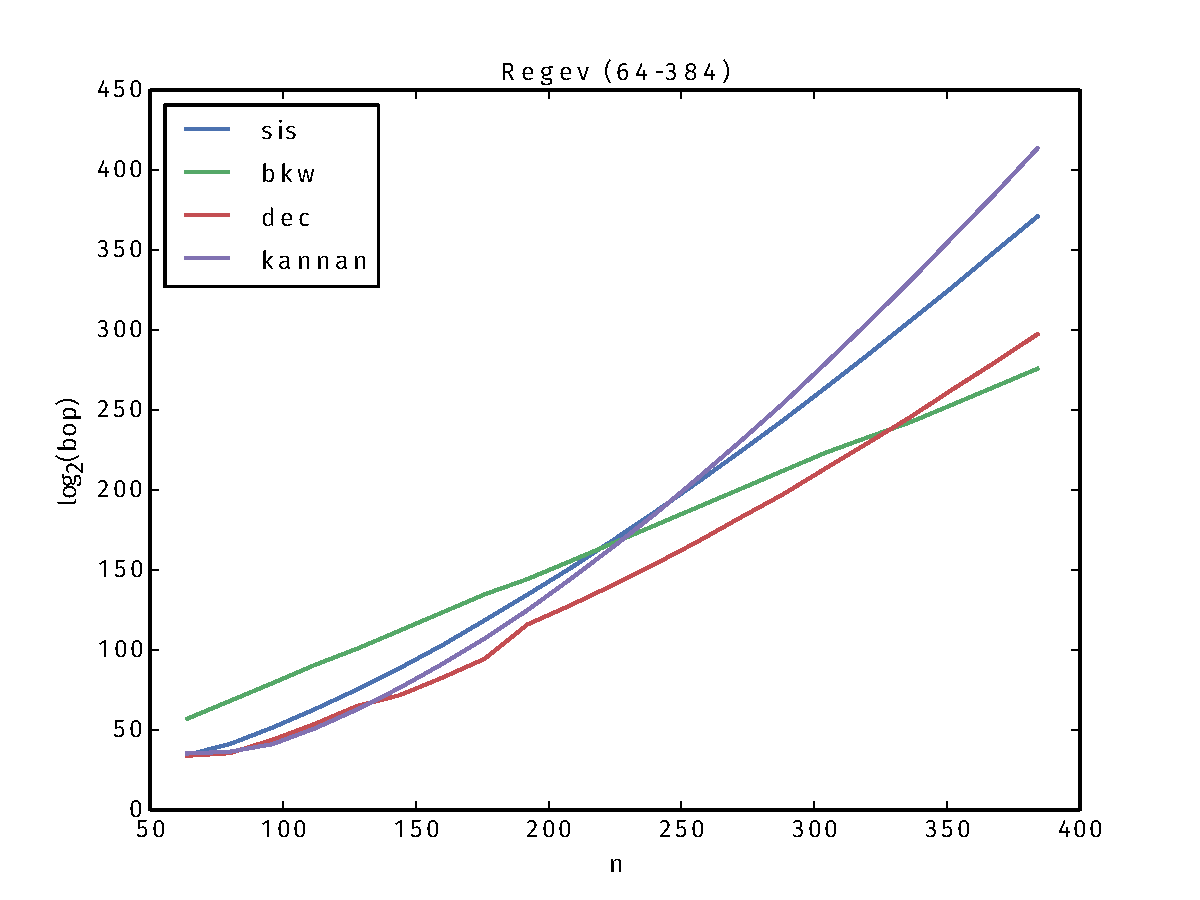
\includegraphics[width=1.0\textwidth]{Regev-64-384.pdf}
\end{frame}

\begin{frame}{Regev: Small Secret}
  \vspace{-1em}
  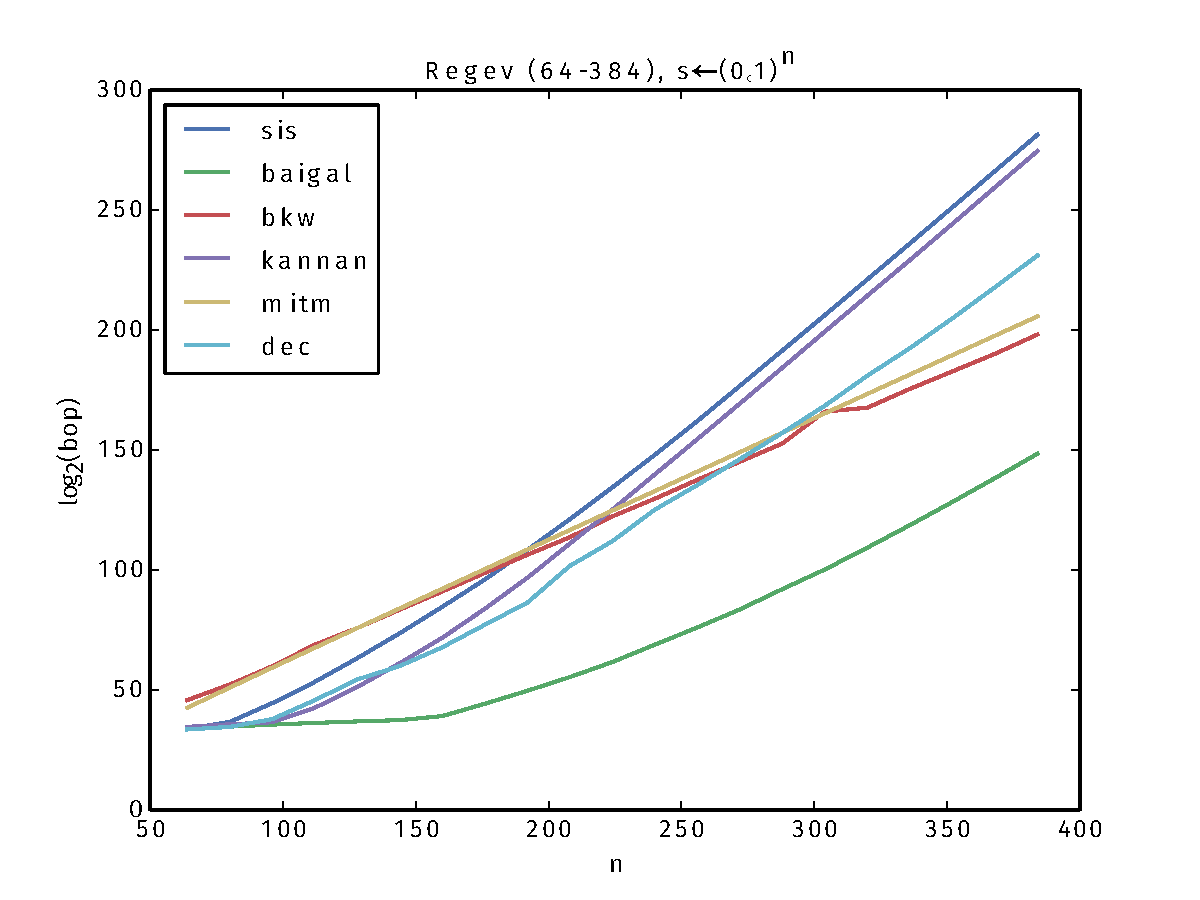
\includegraphics[width=1.0\textwidth]{Regev-(0,1)-64-384.pdf}
\end{frame}


\begin{frame}{FHE}
  \vspace{-1em}
  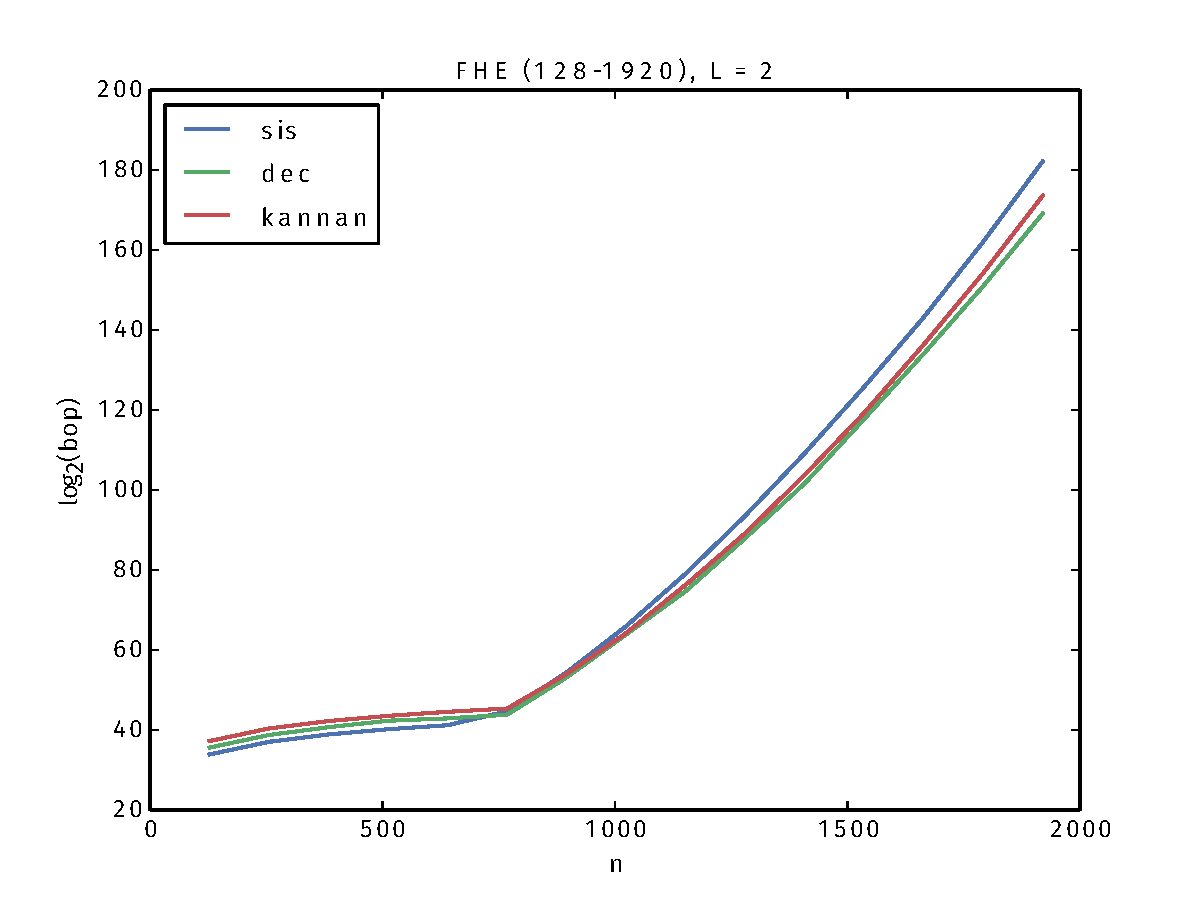
\includegraphics[width=1.0\textwidth]{FHE-2-128-1920.pdf}
\end{frame}

%%%% CONCLUSIONS%%%%%%

\section{Conclusion}


\begin{frame}{So what?}

  \begin{alertblock}{Results}
    \begin{itemize}
    \item No one algorithm always outperforms all others.
    \item Parameters are paramount.
    \item Small secrets matter.
    \end{itemize}
  \end{alertblock}

  \begin{alertblock}{Open Problems}
    \begin{itemize}
    \item Is there an algorithm in $2^{\bigO{n}}$ time but less than $2^{\bigO{n}}$ memory?
    \item How long does lattice reduction actually take?
    \item Can we bridge the gap between theory and practice for small secrets?
    \end{itemize}
  \end{alertblock}
\end{frame}


\begin{frame}{Thank you}
  \centering
  \alert{\Large Questions?} \\
  \vfill
  \begin{description}
  \item[survey] \url{http://eprint.iacr.org/2015/046}
  \item[estimator] \url{https://bitbucket.org/malb/lwe-estimator}
  \end{description}
\end{frame}

\newcommand{\etalchar}[1]{$^{#1}$}

\begin{frame}{Bibliography}
\begin{tiny}
\begin{thebibliography}{AFC{\etalchar{+}}13}
\bibitem[AFC{\etalchar{+}}13]{BB:AFCGS13}
M.A., Robert Fitzpatrick, Daniel Cabracas, Florian Göpfert, and
  Michael Schneider.
\newblock A generator for {LWE} and {Ring-LWE} instances, 2013.
\newblock available at
  \url{http://www.iacr.org/news/files/2013-04-29lwe-generator.pdf}.

\bibitem[AFFP11]{AC:AFFP11}
M.A., Pooya Farshim, Jean-Charles Faug{\`e}re, and Ludovic
  Perret.
\newblock Polly cracker, revisited.
\newblock In Dong~Hoon Lee and Xiaoyun Wang, editors, {\em ASIACRYPT~2011},
  volume 7073 of {\em {LNCS}}, pages 179--196. Springer, December 2011.

\bibitem[BBD09]{PQCBook}
Daniel~J. Bernstein, Johannes Buchmann, and Erik Dahmen, editors.
\newblock {\em Post-Quantum Cryptography}.
\newblock Springer, 2009.

\bibitem[BLP{\etalchar{+}}13]{STOC:BLPRS13}
Zvika Brakerski, Adeline Langlois, Chris Peikert, Oded Regev, and Damien
  Stehl{\'e}.
\newblock Classical hardness of learning with errors.
\newblock In Dan Boneh, Tim Roughgarden, and Joan Feigenbaum, editors, {\em
  45th ACM STOC}, pages 575--584. {ACM} Press, June 2013.

\bibitem[BV11]{FOCS:BraVai11}
Zvika Brakerski and Vinod Vaikuntanathan.
\newblock Efficient fully homomorphic encryption from (standard) {LWE}.
\newblock In Rafail Ostrovsky, editor, {\em 52nd FOCS}, pages 97--106. {IEEE}
  Computer Society Press, October 2011.

\bibitem[GHS12]{C:GenHalSma12FULL}
Craig Gentry, Shai Halevi, and Nigel~P. Smart.
\newblock Homomorphic evaluation of the {AES} circuit.
\newblock {\em {IACR} Cryptology ePrint Archive}, 2012:99, 2012.

\bibitem[GPV08]{STOC:GenPeiVai08}
Craig Gentry, Chris Peikert, and Vinod Vaikuntanathan.
\newblock Trapdoors for hard lattices and new cryptographic constructions.
\newblock In Richard~E. Ladner and Cynthia Dwork, editors, {\em 40th ACM STOC},
  pages 197--206. {ACM} Press, May 2008.
\end{thebibliography}
\end{tiny}
\end{frame}

\begin{frame}{Bibliography}
\begin{tiny}
\begin{thebibliography}{AFC{\etalchar{+}}13}
\bibitem[LP11]{RSA:LinPei11}
Richard Lindner and Chris Peikert.
\newblock Better key sizes (and attacks) for {LWE}-based encryption.
\newblock In Aggelos Kiayias, editor, {\em CT-RSA~2011}, volume 6558 of {\em
  {LNCS}}, pages 319--339. Springer, February 2011.

\bibitem[Reg05]{STOC:Regev05}
Oded Regev.
\newblock On lattices, learning with errors, random linear codes, and
  cryptography.
\newblock In Harold~N. Gabow and Ronald Fagin, editors, {\em 37th ACM STOC},
  pages 84--93. {ACM} Press, May 2005.

\bibitem[Reg09]{DBLP:journals/jacm/Regev09}
Oded Regev.
\newblock On lattices, learning with errors, random linear codes, and
  cryptography.
\newblock {\em J. {ACM}}, 56(6), 2009.

\end{thebibliography}
\end{tiny}
\end{frame}

\end{document}

%%% Local Variables: 
%%% coding: utf-8
%%% mode: latex
%%% TeX-engine: xetex
%%% TeX-master: t
%%% End:
